\scanpage{75}
% archive foliation: 74
\uline{Cor} Conclusion valable dans le cas $\mathrm I$, si
$S'$ est propre sur $S$ et si $\underline W^a(\mathfrak X)$ est loc. noeth.

$\overline{\mathrm M}$ raisonnement que pour $\mathrm I'$.

Mettons ensemble les résultats obtenus.

\uline{Théorème 1} Dans le cas d'un foncteur de Greenberg
\inserted{spécial}, ou d'un foncteur $\underline W_{S'}$ défini
par un morphisme $S'\to S$ fini, loc. libre,
\deleted{\unsure{par}} \unsure{radiciel}, le $W^a(\mathfrak X)$ existe pour
\deleted{\unsure{tout}} préschéma $\mathfrak X$ sur $W(S)$.
\deleted{\unsure{Soit} $\mathfrak X=$}
$W^a$ est de plus un foncteur de \uline{nature locale}.
\margin{\figure{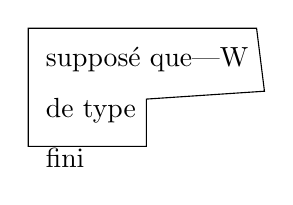
\begin{tikzpicture}[x=1cm,y=1cm]
\node[anchor=west] at (0,1.1) {\unsure{supposé} \unsure{que|W}};
\node[anchor=west] at (0,.45) {\unsure{de type}};
\node[anchor=west] at (0,-.15) {\unsure{fini}};
\draw (-.1,.0)--(-.1,1.5)--(2.8,1.5)--(2.9,.7)--(1.4,.6)--(1.4,.0)--cycle;
\end{tikzpicture}}}

\uline{Théorème 1 bis}
\deleted{Dans le cas $\unsure{\mathrm{II}}$ \unsure{ou} $\unsure{\mathrm I}$, $\mathrm I'$,}
\inserted{Supposons qu'on soit dans le cas $\mathrm I'$.}
\deleted{$\varphi_{S'/S}(\unsure{\mathfrak X})$}
(i) Si $\varphi_{S'/S}(\mathfrak X)$ existe, alors
pour tt ouvert $\mathcal U$ de $\mathfrak X$,
$\varphi_{S'/S}(\mathcal U)$ existe
et $\varphi_{S'/S}(\mathcal U)\to\varphi_{S'/S}(\mathfrak X)$ est une
immersion ouverte.

(ii) Soit $\mathfrak X=\bigcup\mathfrak X_i$, où les $\mathfrak X_i$ sont
tels que pour tt $s\in S$, toute \deleted{\unsure{fibre}}
\inserted{partie finie} de $\mathfrak X_s$ sur $S'_s$ soit contenue dans un $\mathfrak X_i$.
Alors si les $\varphi_{S'/S}(\mathfrak X_i)$ existent, $\varphi_{S'/S}(\mathfrak X)$
